\chapter{Methodology}
\label{ch:Methodology}
This chapter outlines the technical methodology adopted in the development of the system, covering both low-level design and software implementation. The approach prioritizes performance, privacy, and modularity, leveraging hardware accelerators where possible and maintaining efficient control over data flow and execution.


%----------------------
%----------------------
\section{Application Modules and Design}
\label{sec:ApplicationDesignModules}
%----------------------

This section provides an overview of the internal architecture and design principles behind the TLDR desktop application. The application is built with the goal of providing a fast, private, and efficient interface for question-answering and summarization tasks over a user-defined corpus of documents. To achieve this, the design incorporates several performance-aware and hardware-conscious modules, especially tailored for Apple’s M1/M2 architecture.

The TLDR system is structured into modular components, each responsible for a specific functionality in the information processing pipeline. These include embedding generation, context retrieval, vector storage, prompt construction, and output generation via a language model. The workflow between these modules is coordinated to support seamless execution, low latency, and high responsiveness, all while maintaining data privacy by running entirely on-device.


%----------------------
\subsection{Overview}
\label{subsec:AppDesignModules-Overview}
%----------------------
The TLDR application follows a modular architecture where different components are responsible for distinct tasks in the RAG (Retrieval-Augmented Generation) pipeline. Figure~\ref{fig:tldr_modules} illustrates the overall design and the control flow between the modules.

\begin{figure}[H]
    \centering
    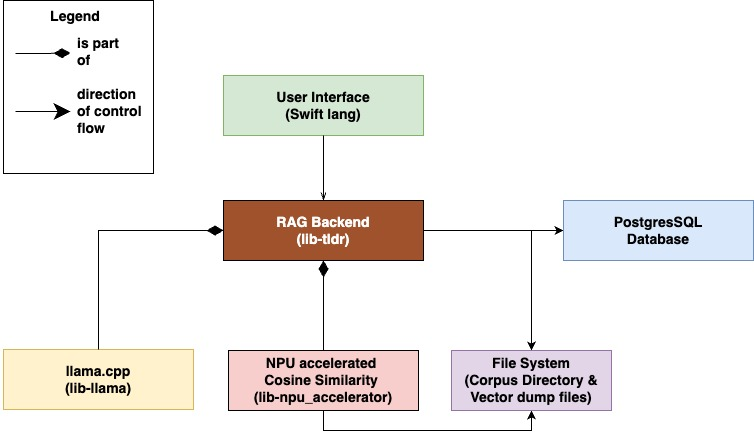
\includegraphics[width=1.0\linewidth]{images/tldr-app-modules.jpg}
    \caption{Modules of TLDR application}
    \label{fig:tldr_modules}
\end{figure}

\begin{itemize}
    \item \textbf{User Interface:} This module provides the graphical frontend for the user. Developed using Swift language for MacOS, it allows users for the users to seamlessly leverage the capabilities of the application. It is responsible for workflows dealing with user experience while delegating all core logic to the backend modules.

    \item \textbf{RAG Backend:} This is the core orchestrator of the application. It manages the full pipeline, including handling user queries, initiating vector search, performing retrieval, and forwarding context to the language model. It communicates with all supporting modules such as the database, NPU based vector search module, llama.cpp and the file system.

    \item \textbf{Database (PostgreSQL):} Stores metadata and document indexing information. It ensures efficient retrieval and persistence of preprocessed documents and vector references. It is plays a crucial role of mapping retrieved vector hashes to their text chunks and document metadata during context retrieval.

    \item \textbf{File System (Corpus Directory and Vector Dump Files):} Contains the document corpus (directory containing source documents) and their corresponding vector dump files. These vector dump are leveraged by the vector search engine using memory-mapped I/O for efficient vector search with low memory overhead.

    \item \textbf{NPU Accelerated Cosine Similarity:} Implements hardware-accelerated cosine similarity by leveraging Apple's Neural Processing Unit (NPU). The backend invokes this module for fast and parallelizable vector cosine similarity computation.

    \item \textbf{llama.cpp:} This module is responsible for language generation i.e LLM inference. It acts as a plugged-in module for the RAG backend and contributes by generating embeddings and chat response during the corresponding stages of the RAG pipeline.
\end{itemize}


%----------------------
\subsection{User Interface}
\label{subsec:AppDesignModules-UI}
%----------------------

The User Interface is in the form of a native MacOS desktop application developed using Swift lang in the Xcode development environment (as depicted in Fig~\ref{fig:tldrGUI}, Fig~\ref{fig:tldrdockicon}). The user interface is designed to be intuitive, lightweight, and self-contained. The application packages all necessary dependencies, including static libraries and LLM weights. enabling fully offline functionality without requiring additional installation or configuration.

The user interface module has the following core purposes:
\begin{itemize}
    \item Provides a clean, chat-style interface where user prompts and LLM responses are displayed as distinct messages to mimic a conversational flow.
    \item Manager all responsibilities regarding user interaction, including persisting user conversation history and any additional user preferences and thereby enable RAG backend to only focus on the RAG functionalities.
    \item \textit{Make a single, self contained portable package that is easy and intuitive to distribute.}
\end{itemize}
\begin{figure}[H]
    \centering
    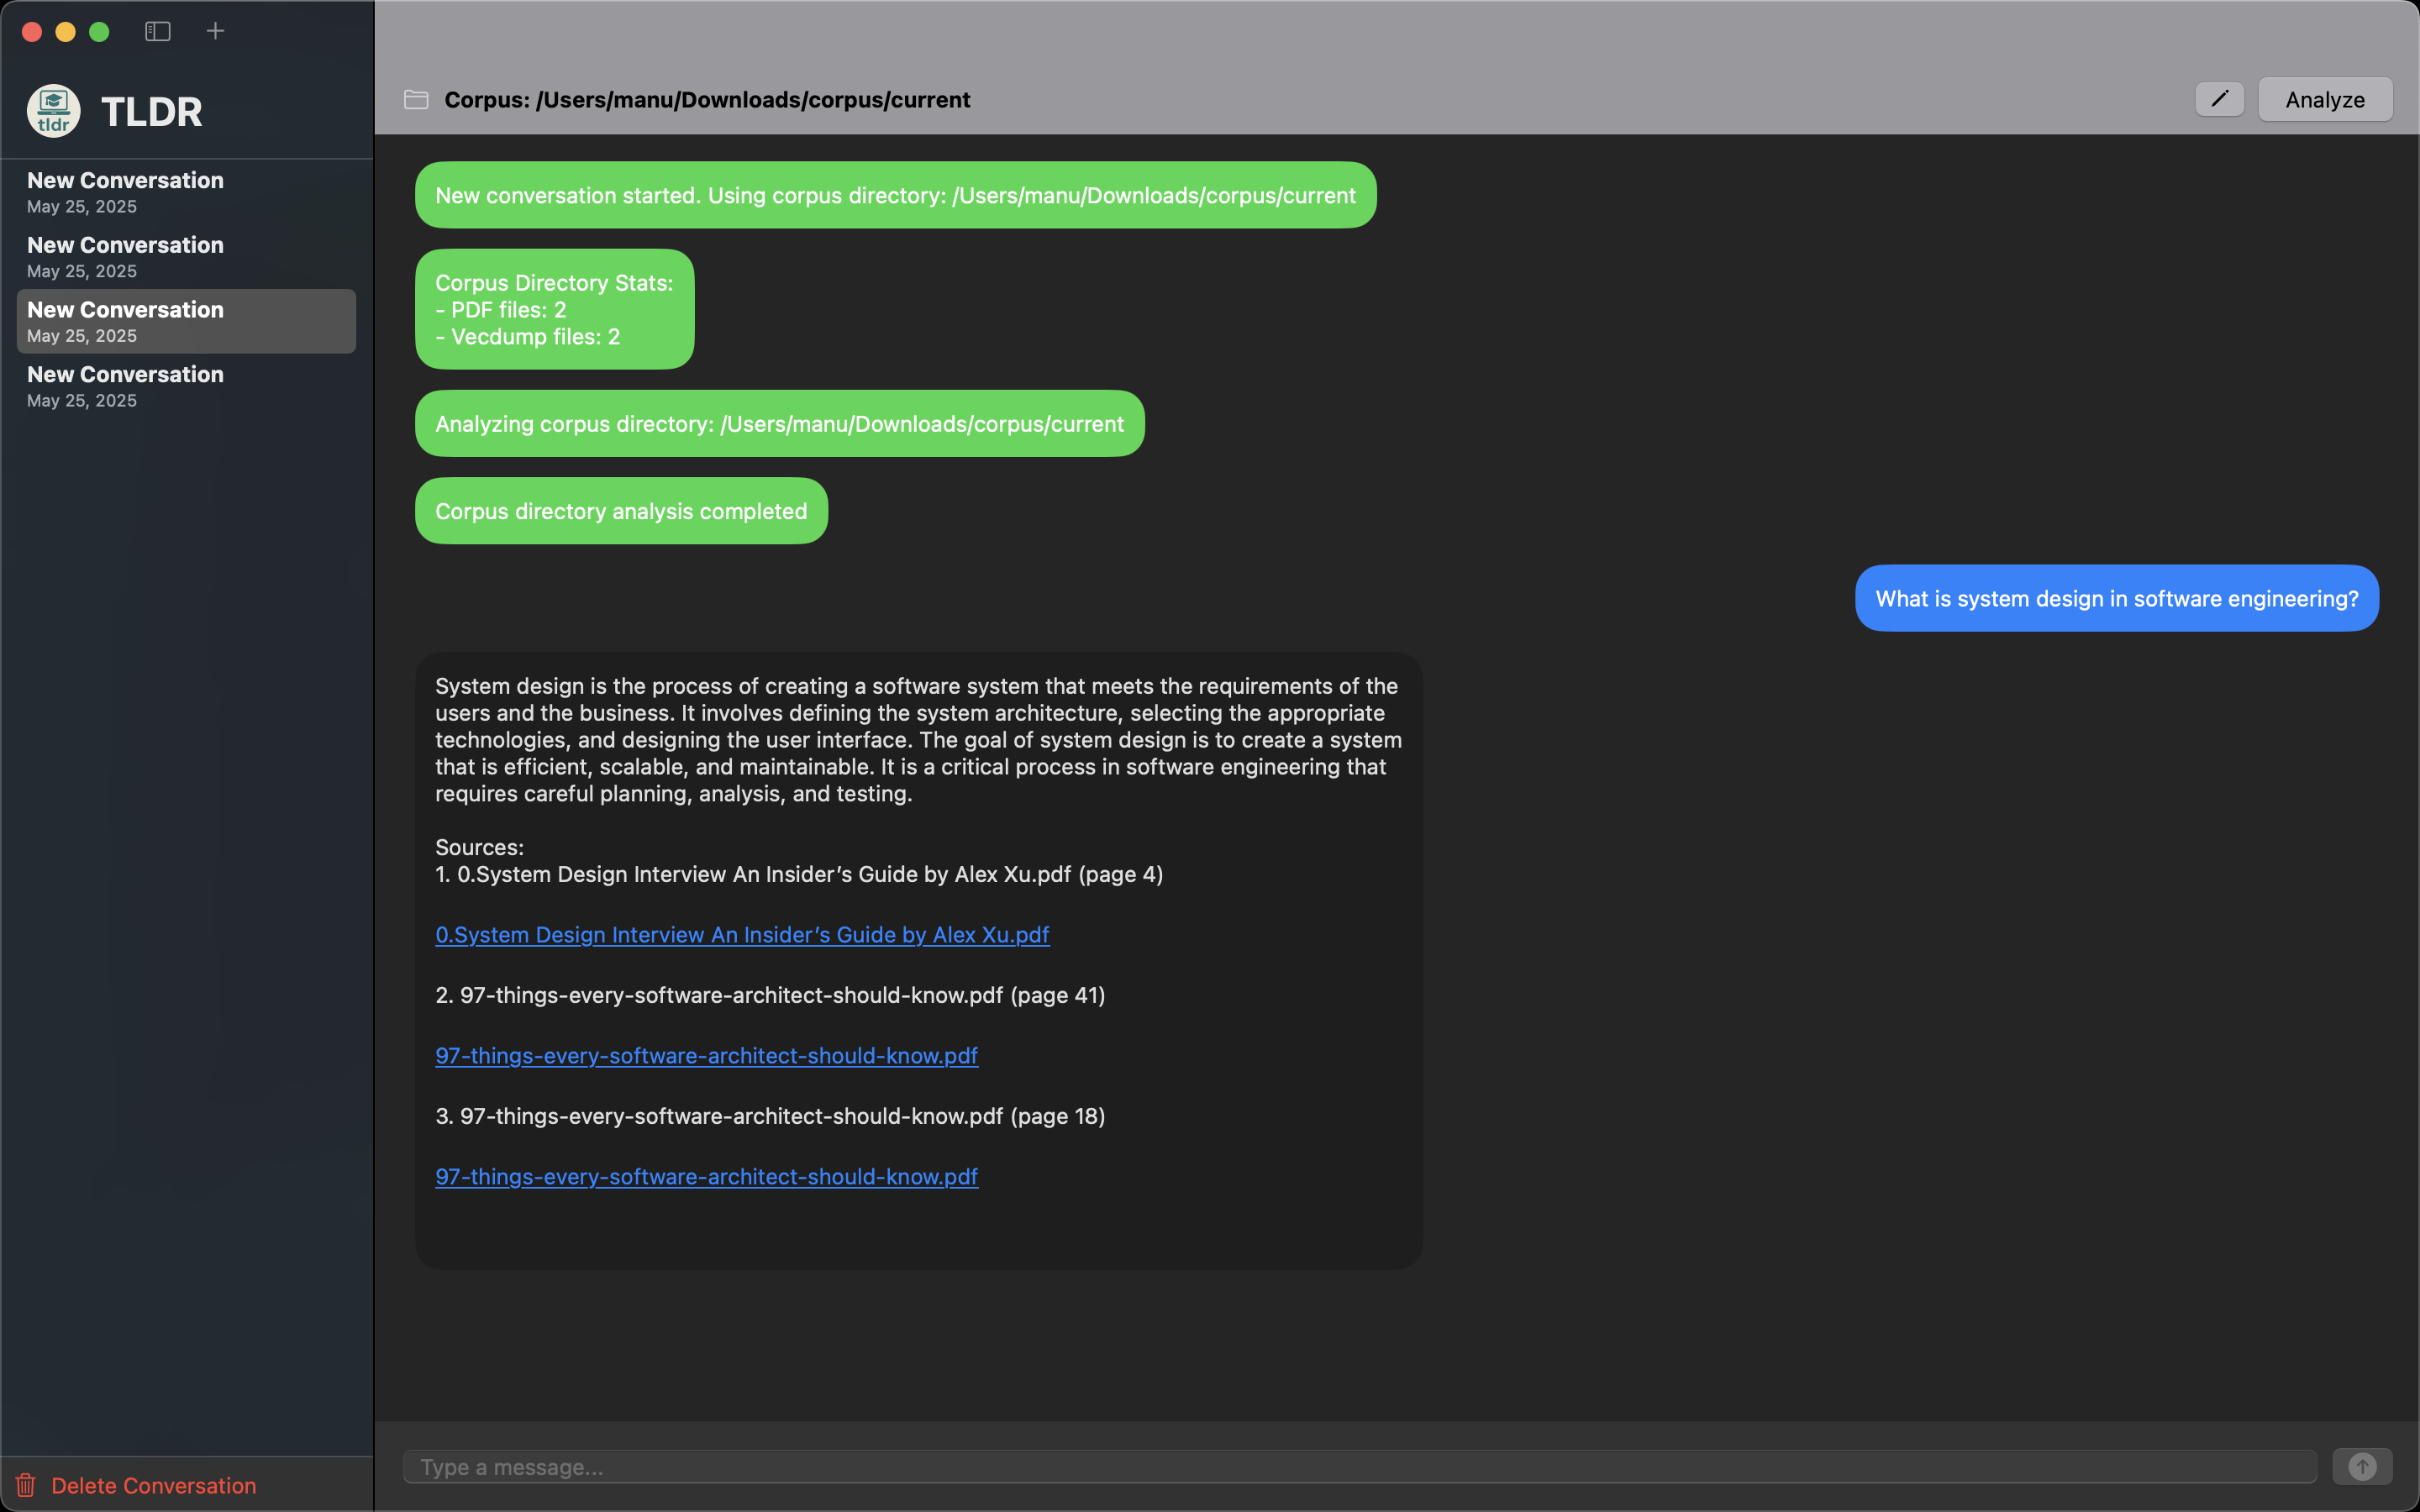
\includegraphics[width=1.0\linewidth]{images/tldr-ui-window.png}
    \caption{Graphical User Interface of TLDR Application}
    \label{fig:tldrGUI}
\end{figure}
\begin{figure}[H]
    \centering
    
\includegraphics[width=0.65\linewidth]{images/tldr-dock-icon.png}
    \caption{TLDR Application Icon as seen in MacOS Dock}
    \label{fig:tldrdockicon}
\end{figure}
%----------------------
\subsubsection{Codebase Organization}
\label{subsubsec:AppDesignModules-UICodebase}
%----------------------

The codebase of the GUI application is illustrated in Figure~\ref{fig:tldrUIFs}. It is organized into several components that serve both core functionality and supporting roles within the application. 
\begin{figure}[H]
    \centering
    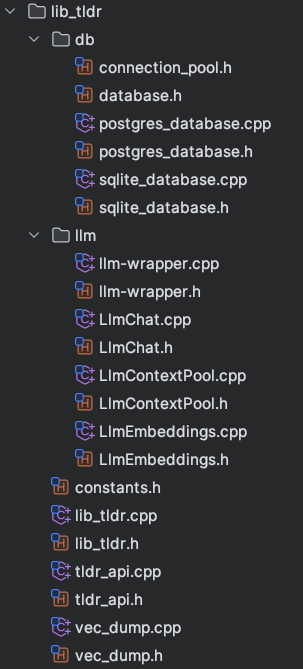
\includegraphics[width=0.5\linewidth]{images/ui-proj-fs.png}
    \caption{UI Project File system}
    \label{fig:tldrUIFs}
\end{figure}
\begin{enumerate}[label=\Alph*.]
    \item \textbf{Overall Structure:}
    \begin{enumerate}[label=\alph*.]
        \item \texttt{tldr}: The Swift language codebase that creates the user interface.
        \item \texttt{TldrAPI}: C++ module with bindings for Swift UI. It serves as a bridge between the Swift UI and the C++ static library of the RAG Backend.
    \item \texttt{artefacts}: Quantized LLM weights and coreml packages, i.e:
    \begin{itemize}
        \item \texttt{Llama-3.2-1B-Instruct-Q3\_K\_L} model for chat
        \item \texttt{all-MiniLM-L6-v2-Q8\_0} model for generating embeddings
        \item \texttt{CosineSimilarityBatched} coreml package for cosine similarity on NPU
    \end{itemize}
    \end{enumerate}

    \item \textbf{UI Architecture (MVVM):}
    \begin{enumerate}[label=\alph*.]
        \item \texttt{tldrApp}: The main SwiftUI entry point where the application lifecycle begins.
        \item \textbf{Models:} Includes \texttt{ConversationData}, \texttt{Message}, and \texttt{RagResultSw} to represent the chat state and RAG outputs. These modules leverage \textit{UserDefaults} a built-in key-value persistance mechanism provided by Apple's Foundation framework to efficiently store and retrieve their information.
        \item \textbf{Views:} Comprises SwiftUI components like \texttt{ChatView} and \texttt{ContentView} to render the main interface.
        \item \textbf{ViewModels:} Contains \texttt{ChatViewModel}, which handles user interaction and backend coordination.
        \item \textbf{Preview Content:} Includes \texttt{Preview Assets} for SwiftUI previews to support development and layout testing.
        \item \textbf{Assets:} Stores static resources such as icons and other UI elements.
    \end{enumerate}
\end{enumerate}
This organization promotes maintainability and allows for clear separation of concerns between UI presentation, interaction logic, and backend communication.
%----------------------
\subsection{RAG Backend}
\label{subsec:AppDesignModules-RAG Backend}
%----------------------
\begin{figure}[htbp]
  \centering
  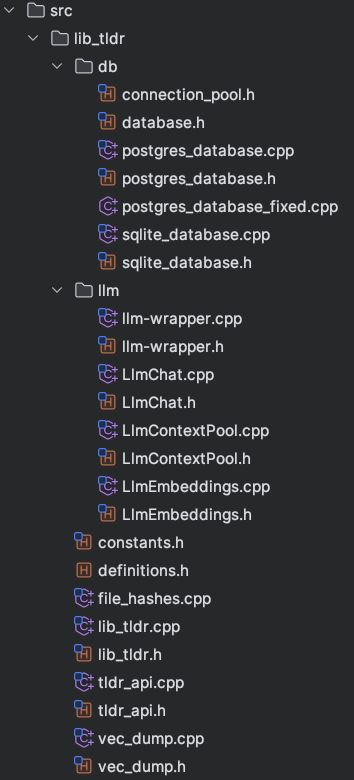
\includegraphics[width=0.5\linewidth]{images/lib_tldr_fs.png}
  \caption{RAG Backend(lib\_tldr) codebase}
  \label{fig:libTldrCodebase}
\end{figure}

The RAG backend is implemented as a C++ static library named \texttt{lib\_tldr}. It serves as the backbone for all core functionalities of the project. This module encapsulates the complete RAG pipeline logic and integrates essential components such as the large language model for text and embedding generation, the vector dump generator and reader, database and file system handlers for storage, and the cosine similarity-based vector retriever (as seen in Fig~\ref{fig:libTldrCodebase}).

The architecture emphasizes modularity and resource efficiency, enabling plug-and-play replacement or extension of components. It adheres to the SOLID principles of object-oriented programming, promoting adaptability, maintainability, and scalability.



Following are the logical sub-modules of RAG Backend:
\begin{enumerate}[label=\Alph*.]
\item{\textbf{Language Model Interface:}}

The system utilizes \texttt{llama.cpp} as the backend for both text generation and embedding extraction. Following components facilitate this integration:

\begin{enumerate}
    \item \textbf{\texttt{LlmChat.cpp \& .h}}: Manage the logic to take user input and retrieved context and generate a response from the chat LLM. 
    \item \textbf{\texttt{LlmEmbeddings.cpp \& .h}}: These modules extract dense vector representations (embeddings) from document chunks, which are subsequently used for semantic similarity search and retrieval.
    \item \textbf{\texttt{LlmContextPool.cpp \& .h}}: These components manage the lifecycle of LLM context objects, which encapsulate the model state necessary for efficient inference. Since LLMs typically require a context to maintain internal buffers, tokenizer state, and memory allocations, it is computationally expensive to initialize a new context for every query or embedding operation. By pooling and reusing contexts across multiple operations, the system significantly reduces initialization overhead and ensures smoother, low-latency performance during both chat and embedding workflows.
    \item \textbf{\texttt{Llm-Wrappers.cpp \& .h}}: Takes care of initializing and cleaning up resources related to the LLMs. It initializes common ggml backend for Apple metal and setting up LLM context pools and initialize Chat and Embedding LLMs by loading their weights into memory.
\end{enumerate}

\item{\textbf{Database Interaction:}}
All persistent storage is handled via the PostgreSQL backend, though an optional SQLite backend is also implemented (but not currently utilized). The database interaction is managed within the \texttt{db} submodule, which includes the follwing:

\begin{enumerate}[label=\alph*.]
\item \textbf{\texttt{database.h}}\: Defines an abstract class that enforces a uniform interface for any underlying database implementation. This design allows the RAG codebase to remain unchanged when switching between different database technologies.
    \item \textbf{\texttt{postgres\_database.cpp \& .h}}: These files handle database initialization, schema definition, and CRUD operations related to documents and embeddings in PostgreSQL Database.
    \item \textbf{\texttt{connection\_pool.h}}: Provides a lightweight connection pooling mechanism to manage multiple concurrent database sessions efficiently. This is especially beneficial during large-scale embedding operations where multiple inserts are performed rapidly. It is efficient to store readily available connections and re-use them instead of creating a new connection for every db interaction.
\end{enumerate}

The PostgreSQL schema stores both high-level document metadata (e.g., title, author, page count) and low-level embedding-related information (e.g., text chunk, hash, embedding vector, page number, and timestamps).

\item{\textbf{Embeddings Vector Storage and Retrieval\:}}

\texttt{vec\_dump.cpp \& .h}  are responsible for managing the serialized storage of raw vector data ("vecdumps"). These are binary representations of embedding vectors that can be rapidly accessed and processed.

Additionally, the system incorporates a hardware-accelerated module referred to as the \texttt{npu-accelerator}, which leverages macOS’s Neural Engine to perform cosine similarity search over large sets of embeddings. This offloads compute-intensive operations from the CPU, enabling real-time retrieval performance on resource-constrained devices.

\item{\textbf{Core Workflow:}}
The \texttt{lib\_tldr.cpp \& .h} contain the core logic that glues the entire system together such as:
\begin{itemize}
    \item Initializing the LLMs and the Database tables (when necessary)
    \item Creating DB connection pool and LLM context pool
    \item Checking for changes in the corpus directory and embedding new documents
    \item Performing Retrieval Augmented Generation
    \item Cleaning up and releasing acquired resources
\end{itemize}


\item{\textbf{RAG Backend API:}}
While the backend contains numerous functions and data structures for internal logic, a clean and minimalistic API (Application Program Interface) is exposed. This allows its client modules (such as the UI module) to leverage its capabilities without being closely coupled with the internal mechanisms of the library.

The \texttt{tldr\_api.cpp \& .h} files expose a clean, C-style API interface for the user-facing application layer on top of the functions present in \texttt{lib\_tldr.cpp \& .h}. 

\end{enumerate}

 %----------------------
\subsection{Database (PostgreSQL)}
\label{subsec:AppDesignModules-DatabasePSQL}
%----------------------
\begin{lstlisting}
CREATE TABLE IF NOT EXISTS documents (
    id UUID PRIMARY KEY DEFAULT uuid_generate_v4(),
    file_hash TEXT NOT NULL UNIQUE,
    file_path TEXT NOT NULL,
    file_name TEXT NOT NULL,
    title TEXT,
    author TEXT,
    subject TEXT,
    keywords TEXT,
    creator TEXT,
    producer TEXT,
    page_count INTEGER,
    created_at TIMESTAMP WITH TIME ZONE DEFAULT CURRENT_TIMESTAMP,
    updated_at TIMESTAMP WITH TIME ZONE DEFAULT CURRENT_TIMESTAMP
);
\end{lstlisting}
\begin{figure}[H]
    \centering
    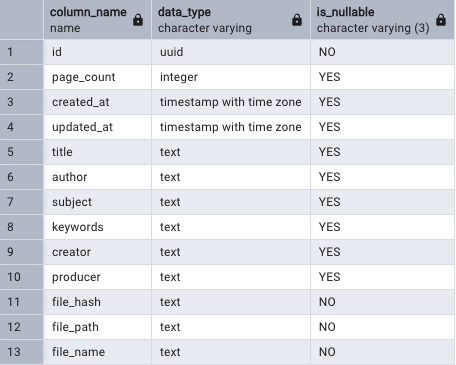
\includegraphics[width=1.0\linewidth]{images/dbtable-documents.png}
    \caption{RAG Output evaluation metrics ~\cite{cardenas2023rag}}
    \label{fig:autoregressive_decoding}
\end{figure}


\begin{lstlisting}
CREATE TABLE IF NOT EXISTS embeddings (
    id BIGSERIAL PRIMARY KEY,
    document_id UUID REFERENCES documents(id) ON DELETE CASCADE,
    chunk_text TEXT NOT NULL,
    embedding_hash TEXT,
    embedding vector(EMBEDDING_SIZE) NOT NULL, 
    page_number INTEGER DEFAULT 0,
    created_at TIMESTAMP WITH TIME ZONE DEFAULT CURRENT_TIMESTAMP
);
\end{lstlisting}
\begin{figure}[H]
    \centering
    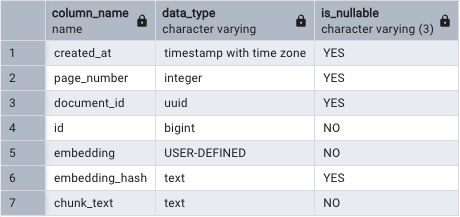
\includegraphics[width=1.0\linewidth]{images/dbtable-embeddings.png}
    \caption{RAG Output evaluation metrics ~\cite{cardenas2023rag}}
    \label{fig:autoregressive_decoding}
\end{figure}
%----------------------
\subsection{File System: Corpus Directory and Vectordump Files}
\label{subsec:AppDesignModules-FSandVectordump_files}
%----------------------
Vector dump files are binary data structures designed for efficient storage of document embeddings. For each input document, a corresponding vector dump file is created. Each such file contains embedding vectors generated from text chunks along with their corresponding MD5 hashes. This format enables fast similarity search and content verification in document retrieval systems.

%----------------------
\subsubsection{Corpus Directory}
\label{subsec:AppDesignModules-CorpusDir}
%----------------------


%----------------------
\subsubsection{Vectordump Files}
\label{subsec:AppDesignModules-Vectordump_FileStructure}
%----------------------
The vector dump file follows a sequential binary layout consisting of three main components: a metadata header, followed by embedding data, and finally hash data. This structure allows for efficient random access to embeddings while maintaining data integrity through hash verification. Hash is also further used for fetching the corresponding text chunk after similar vectors are obtained for a query.

   \begin{figure}[H]
    \centering
    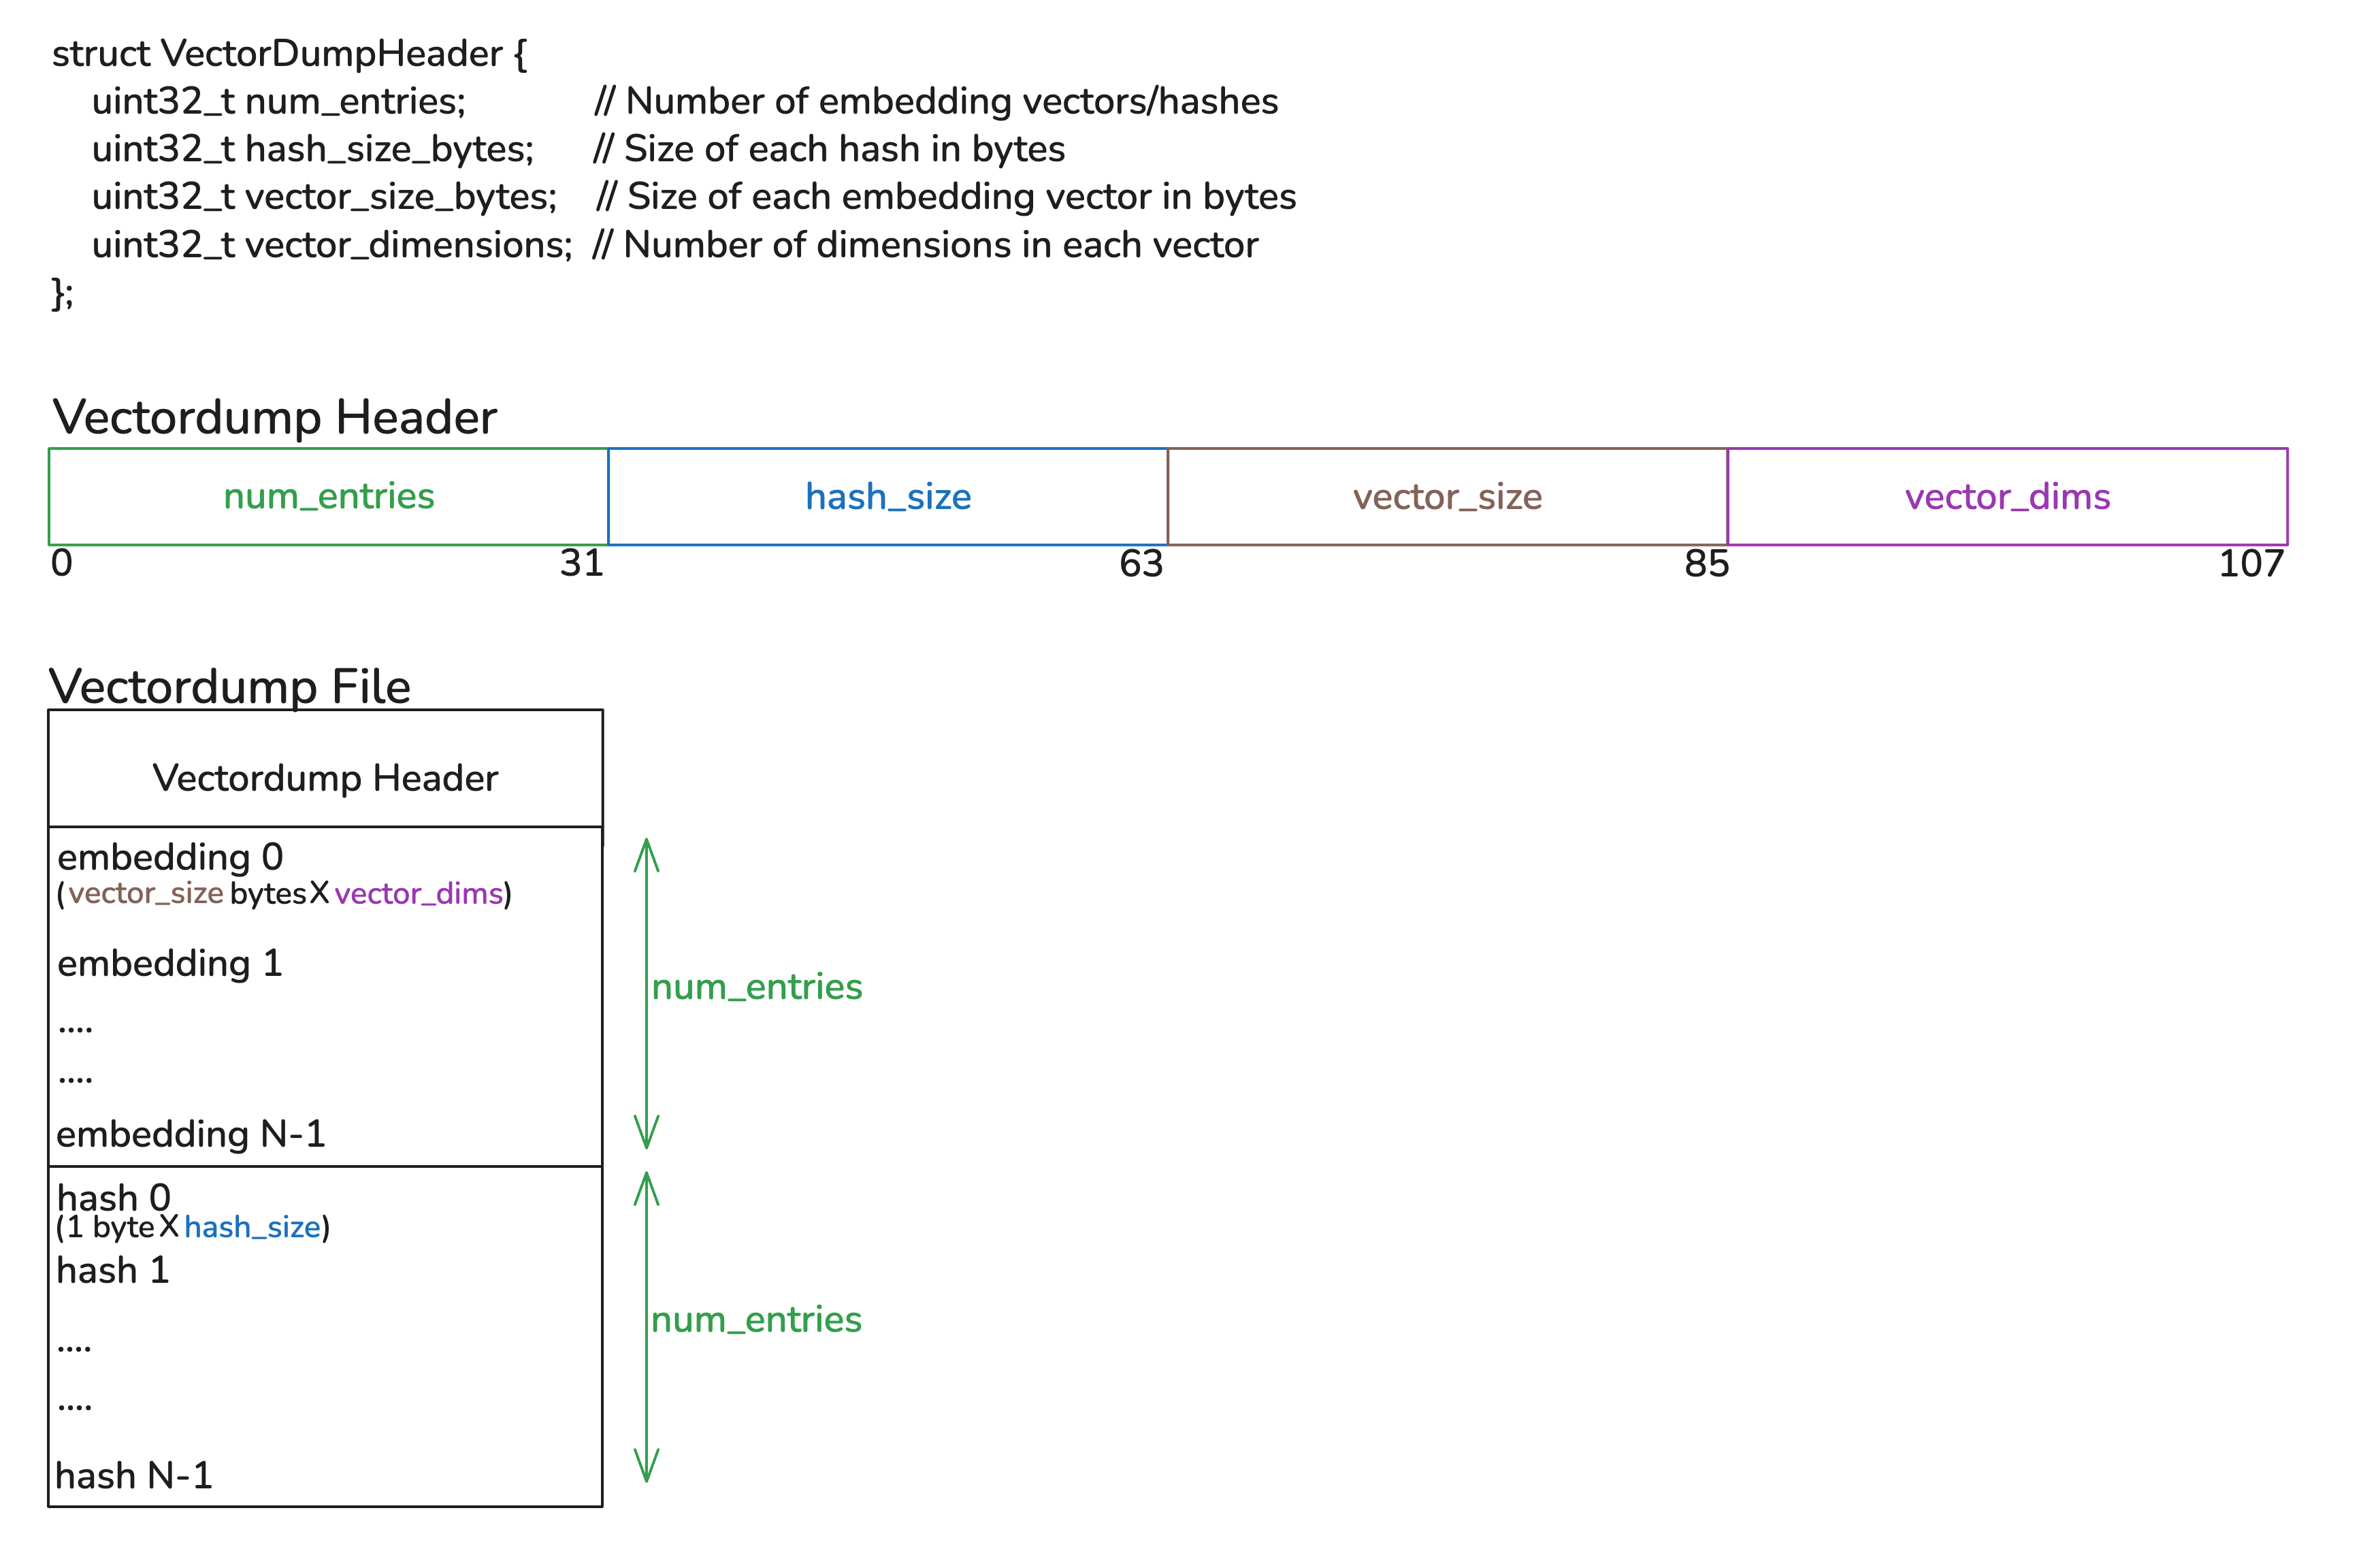
\includegraphics[width=1.0\linewidth]{images/VectorDumpFiles.png}
    \caption{Vector dump file structure}
    \label{fig:vectordumpfilestructure}
\end{figure}

%----------------------
\subsubsection{Vectordump Header}
\label{subsec:AppDesignModules-Vectordump_Header}
%----------------------
In order to process the vector dump file, the header is first read and the necessary information is obtained regarding the data layout in the file. The information is arranged in the layout as illustrated in Figure~\ref{fig:vectordumpfilestructure}. The elements are as follows:
\begin{itemize}
    \item \texttt{num\_entries} - Total number of embedding/hash pairs stored in the file
    \item \texttt{hash\_size\_bytes} - Size of each MD5 hash in bytes (always 16 for standard MD5)
    \item \texttt{vector\_size\_bytes} - Total byte size of each embedding vector
    \item \texttt{vector\_dimensions} - Number of floating-point dimensions per embedding vector
\end{itemize}

The header is read by pointing the $VectorDumpHeader$ struct to the memory location of the loaded file. This helps obtain the  necessary information required to access the data sections of the file.

%----------------------
\subsubsection{Data Sections}
\label{subsec:Vectordump_DataSections}
%----------------------
Once the header section is loaded, the data obtained is then used for calculating the memory locations of the embedding and hash arrays.
Pointers are used to access these locations to simulate the structure of an array on top of raw binary data read into the memory. This approach is simple and efficient and prevents needless memory allocations and data copies.

\textbf{Embeddings:} Contains $N$ consecutive embedding vectors, where $N$ = \texttt{num\_entries}. Each vector occupies \texttt{vector\_size\_bytes} and represents a \texttt{vector\_dimensions}-dimensional embedding, typically stored as 32-bit floating-point values.

\textbf{Hashes:} Contains $N$ consecutive MD5 hash values, each exactly 16 bytes. However, the smallest unit of storage is of $uint64_t$ type, i.e., units of 2 bytes. Hence, a 16 byte MD5 hash would have a hash size of 8. The hash at index $i$ corresponds to the MD5 digest of the original text chunk used to generate \texttt{embedding[i]}.


%----------------------
\subsubsection{Data Relationship}
\label{subsec:Vectordump_DataRelationship}
%----------------------

The file maintains strict positional correspondence: for any index $i \in [0, N-1]$, \texttt{embedding[i]} and \texttt{hash[i]} represent the same document chunk. This one-to-one mapping enables efficient lookup operations and integrity verification during retrieval.

The data is used as follows:
\begin{enumerate}[label=\arabic*.]
\item Load the first half of the file in memory using \textbf{mmap} and perform cosine similarity search.
    \item Obtain index of the top $K$ relevant vectors from Cosine similarity module.
    \item Fetch the hash values at the obtained indices.
    \item Query the database for text chunks associated with the hash values.
\end{enumerate}
    
This design allows for prioritized access to necessary data and its direct usage for cosine similarity search with no further processing or data manipulations, allowing for an efficient search through the entire corpus.




User Interface RAG Backend  PostgreSQL Database NPU Accelerated Cosine Similarity 
%----------------------
\subsection{NPU Accelerated Cosine Similarity}
\label{subsec:AppDesignModules-NpuCosineSim}
%----------------------
(lib-npu\_accelerator)
\begin{figure}[H]
    \centering
    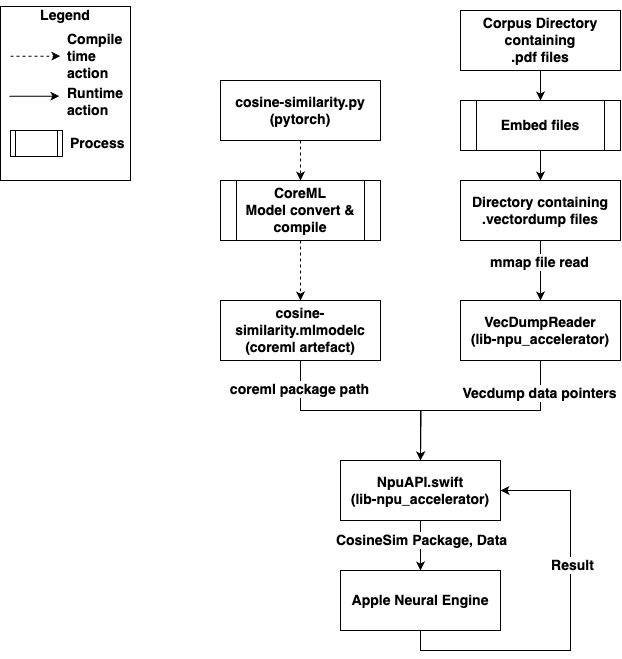
\includegraphics[width=0.8\linewidth]{images/npu-accelerator-module-worklfow.jpg}
    \caption{RAG Output evaluation metrics ~\cite{cardenas2023rag}}
    \label{fig:autoregressive_decoding}
\end{figure}

\subsection{NPU Accelerator Module}

The NPU accelerator module is a specialized component of the TLDR macOS desktop application that leverages Apple's Neural Processing Unit to perform hardware-accelerated cosine similarity computations for Retrieval-Augmented Generation (RAG) workflows. The module serves as a bridge between document processing, vector similarity computation, and language model integration, utilizing Apple's dedicated neural processing hardware to optimize performance. By integrating llama.cpp for embedding generation and chat functionality, the system enables efficient document processing and semantic search capabilities specifically optimized for Apple Silicon devices with Neural Engine support.

\subsubsection{Processing Workflow}
\begin{figure}[H]
    \centering
    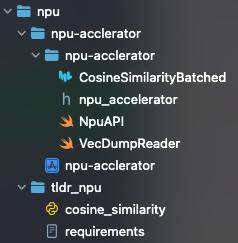
\includegraphics[width=0.8\linewidth]{images/npu-fs.png}
    \caption{RAG Output evaluation metrics ~\cite{cardenas2023rag}}
    \label{fig:autoregressive_decoding}
\end{figure}

The NPU accelerator follows a comprehensive dual-pipeline processing workflow as illustrated in the system diagram. The left pipeline begins with a PyTorch-based cosine-similarity.py implementation that serves as the foundation for similarity computations. This PyTorch model undergoes a CoreML model conversion and compilation process, transforming the original implementation into an optimized CoreML artifact specifically designed for Apple's Neural Engine execution. The compilation step produces the cosine-similarity.mlmodelc package, which contains the optimized model ready for hardware acceleration.

The right pipeline operates in parallel, handling document processing and vector storage. PDF files from a designated corpus directory are processed through an embedding generation system that creates high-dimensional vector representations of the document content. These embeddings are systematically stored in a directory containing vectordump files, which serve as the persistent storage layer for the vector data. The vectordump files are designed for efficient access through memory mapping techniques.

During runtime operations, the VecDumpReader component, powered by the lib-npu\_accelerator library, accesses the vectordump files through memory mapping (mmap file read) operations. This approach provides efficient access to vector data without loading entire datasets into memory. The VecDumpReader extracts vectordump data pointers that reference specific vector locations within the mapped memory space.

The workflow convergence occurs at the NpuAPI.swift interface, which acts as the central coordination point between the two processing pipelines. This Swift-based API receives input from both the CoreML package data (containing the optimized similarity computation model) and the vectordump data pointers (referencing the document embeddings). The NpuAPI facilitates communication with Apple's Neural Engine, orchestrating the hardware-accelerated cosine similarity computations between query vectors and the stored document embeddings. The final output consists of similarity scores that enable the RAG system to identify and retrieve the most relevant document segments for generating contextually appropriate responses.

\subsubsection{File Structure}
BRIDGE TO NPU API AND C++ API
The module is organized into a hierarchical structure within the main npu-accelerator directory, reflecting the different functional components of the system. At the top level, the CosineSimilarityBatched.h header file defines interfaces for batched similarity operations, enabling efficient processing of multiple similarity computations in parallel. The core npu\_accelerator directory contains the primary implementation files that handle the low-level neural processing operations and coordinate with the Apple Neural Engine.

The NpuAPI directory houses the Swift interface components responsible for bridging between the CoreML models and the Neural Engine hardware. This component provides the primary API surface for the broader TLDR application to interact with the NPU acceleration capabilities. The VecDumpReader directory contains specialized components for handling vector data access operations, including memory mapping functionality and efficient data pointer management for large-scale vector datasets.

Supporting the main implementation are several auxiliary files that facilitate development and deployment. The cosine\_similarity.py script serves as the original PyTorch implementation and provides utilities for model preparation and conversion to CoreML format. The requirements.txt file specifies the necessary Python dependencies required for the model conversion pipeline and any associated preprocessing operations. This file structure reflects a clear separation of concerns between hardware acceleration interfaces, vector data management, model conversion utilities, and dependency management.
%----------------------
\subsection{llama.cpp}
\label{subsec:AppDesignModules-LLaMaCpp}
%----------------------
(lib-llama)

uses a fork of llama.cpp with minor modifcations to strip down build script to focus to build a static library for macos with ggml metal backend

fork located at https://github.com/manuhg/llama.cpp

uses functions exposed via llama.h and ggml.h to perform tokenization,  decoding and sampling

LLmChat and LLmEmbedding are based on workflows seen in llama.cpp's server.cpp and embedding.cpp files Uses \textbf{openmp} for optimizing the tokenization and batch decoding process

%----------------------
%----------------------
\section{Application Design - Workflow Overview}
\label{subsec:AppDesignWorkflow-Overview}
%----------------------

\begin{figure}[H]
    \centering
    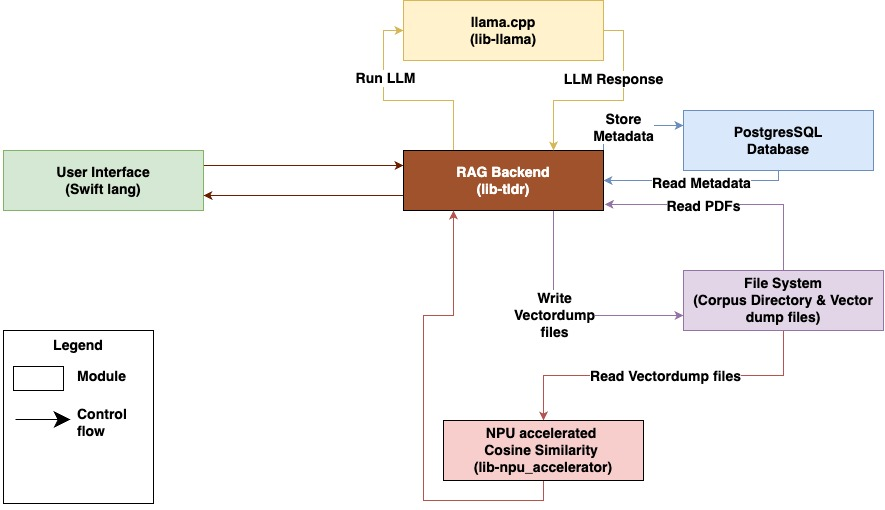
\includegraphics[width=1.0\linewidth]{images/tldr-app-module-interactions.jpg}
    \caption{RAG Output evaluation metrics ~\cite{cardenas2023rag}}
    \label{fig:autoregressive_decoding}
\end{figure}



Figure~\ref{fig:tldr_workflow} illustrates the end-to-end workflow of the TLDR application. It is divided into three primary phases: system initialization, document corpus embedding, and query-based retrieval-augmented generation (RAG).

%----------------------
\subsubsection{System Initialization}
\label{subsec:AppDesignWorkflow-SystemInitialization}
%----------------------

\begin{figure}[H]
    \centering
    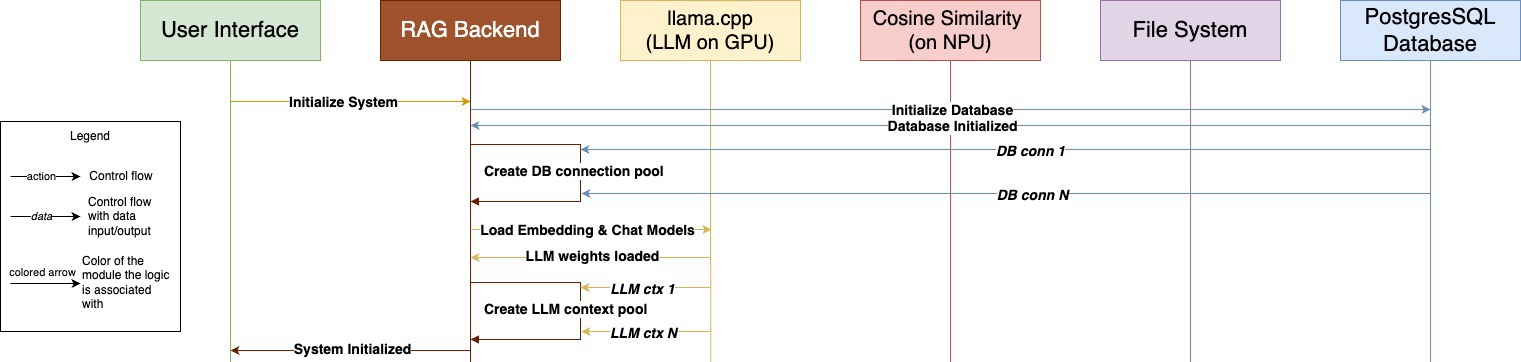
\includegraphics[width=1.0\linewidth]{images/tldr-app-worklfow-pt1.jpg}
    \caption{RAG Output evaluation metrics ~\cite{cardenas2023rag}}
    \label{fig:autoregressive_decoding}
\end{figure}


The initialization phase sets up the backend infrastructure and prepares the application for use. This includes:

\begin{itemize}
    \item The user launches the application, triggering the backend.
    \item The \textbf{RAG Backend} initializes a connection pool to the \textbf{PostgreSQL Database}.
    \item The LLM weights and context pools are loaded via \texttt{llama.cpp}, enabling multi-threaded inference.
    \item Cosine similarity routines are prepared via the \textbf{NPU accelerator} module.
    \item System status is communicated back to the \textbf{User Interface}, indicating readiness.
\end{itemize}


%----------------------
\subsubsection{Embedding the Corpus}
\label{subsec:AppDesignWorkflow-EmbeddingCorpus}
%----------------------

\begin{figure}[H]
    \centering
    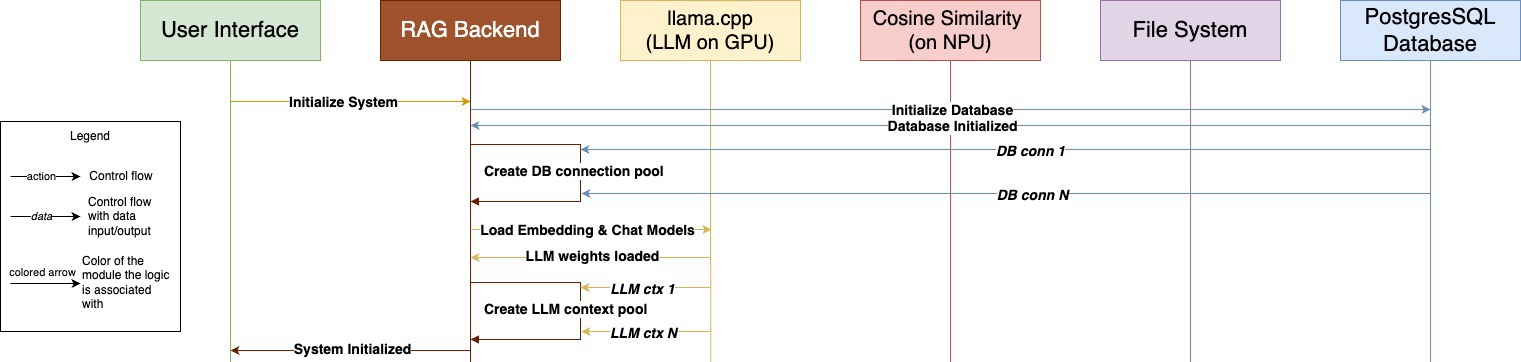
\includegraphics[width=1.0\linewidth]{images/tldr-app-worklfow-pt1.jpg}
    \caption{RAG Output evaluation metrics ~\cite{cardenas2023rag}}
    \label{fig:autoregressive_decoding}
\end{figure}

When a user specifies a directory to embed:

\begin{itemize}
    \item The \textbf{RAG Backend} scans the specified directory for documents using the File System.
    \item Each document is loaded, chunked, and converted to embeddings using a pre-defined embedder.
    \item Embeddings, text chunks, and associated metadata are inserted into the \textbf{PostgreSQL Database}.
    \item In parallel, the backend also writes a vector dump file to the \textbf{File System}, which stores the hash of each vector for quick access.
\end{itemize}

This dual-storage mechanism (DB + mmap vector cache) allows fast retrieval during inference while maintaining queryable metadata.


%----------------------
\subsubsection{Performing RAG}
\label{subsec:AppDesignWorkflow-PerformingRAG}
%----------------------


\begin{figure}[H]
    \centering
    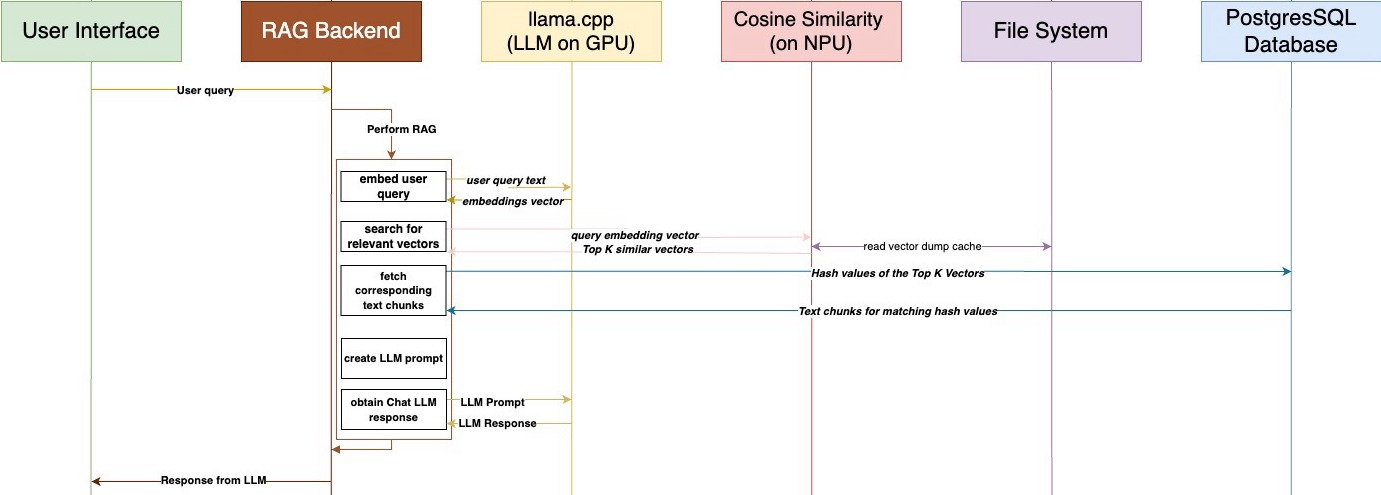
\includegraphics[width=1.0\linewidth]{images/tldr-app-worklfow-pt3.jpg}
    \caption{RAG Output evaluation metrics ~\cite{cardenas2023rag}}
    \label{fig:autoregressive_decoding}
\end{figure}

Once the corpus is embedded, the user may input a query. The following steps are executed:

\begin{itemize}
    \item The user query is embedded using the same embedding model.
    \item The embedded query vector is sent to the \textbf{Cosine Similarity} module running on the NPU.
    \item A top-$k$ similarity search is performed against memory-mapped vector files using the NPU, returning hash values of the best matches.
    \item These hashes are used to retrieve the corresponding text chunks from the \textbf{PostgreSQL Database}.
    \item A prompt is constructed and sent to the \textbf{LLM} via \texttt{llama.cpp}.
    \item The generated response is sent back to the \textbf{User Interface}.
\end{itemize}

This phase exemplifies the retrieval-augmented generation paradigm, grounded entirely in the user’s local corpus and executed with optimized hardware utilization.

